\section{Sprints}\label{sec:sprints}

In this section we will show the sprint backlogs and sprint burndown charts for every sprint of the project, focusing on one sprint at a time and explaining it in detail.

\subsection{Sprint 1}

The theme of the sprint was documentation, since a lot of reports were due during this sprint. The theme also included getting introduced to the project and getting to know the tools required.

Some of the things that went well were that we finished every story on the sprint backlog, getting to know the project went well since Þór Adam Rúnarsson, a previous project member, provided good hand-off information to us.

The things that did not go so well were that we underestimated the size of most of the stories, specifically the ones related to documentation. These stories should have been rated higher, since we ended up spending a lot of time on them. We also wasted too much time on technical difficulties, such as getting access to the version control system. 


\begin{figure}[H]
	\centering
	\graphicspath{ {./graphics/} }
    \centerline{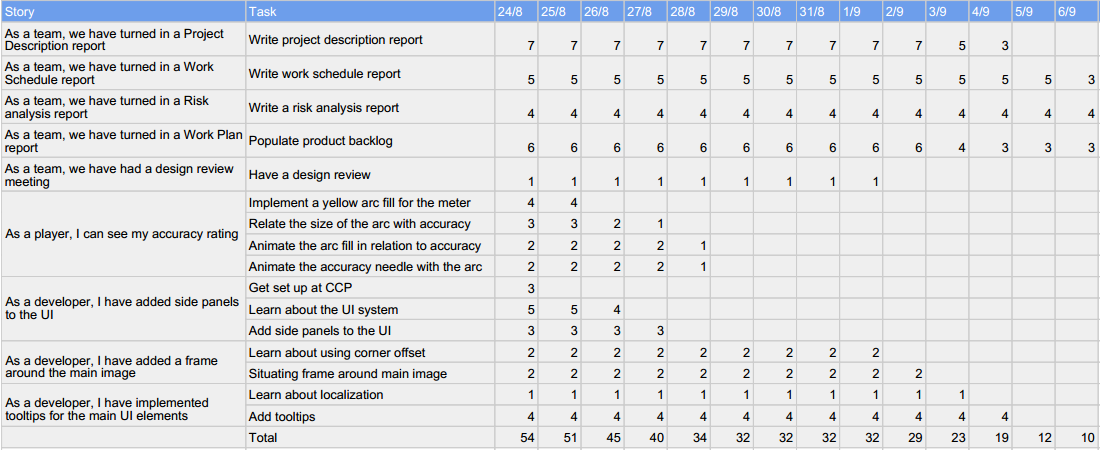
\includegraphics[scale=0.65]{sprint1.PNG}}
    \caption{\label{fig:s1}Sprint backlog for sprint 1}
\end{figure}

\begin{figure}[H]
	\centering
	\graphicspath{ {./graphics/} }
    \centerline{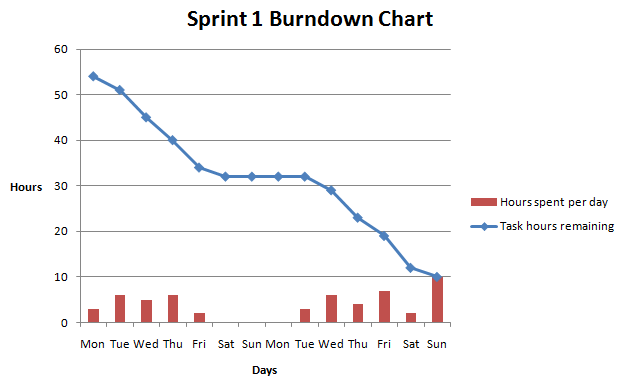
\includegraphics[scale=0.8]{sprint1bdc.PNG}}
    \caption{\label{fig:s1bd}Sprint burndown chart for sprint 1}
\end{figure}

\subsection{Sprint 2}
The theme of the sprint was fixing errors, optimization and improving documentation.

The things that went well in this sprint were that we managed to fix all errors and we were able to optimize the game. 

Some of the things that did not go so well were that we had to spend a lot of time improving our documentation. We also put a story (implementing an interactive tutorial phase for the game) on the sprint backlog that we should have realized was too big to be able to finish during the sprint. We should have broken that story up into smaller stories to give us a better view of our velocity per sprint. Because of those two factors we were unable to finish the large story and one other story, therefore our velocity didn't look too good.

\begin{figure}[H]
	\centering
	\graphicspath{ {./graphics/} }
    \centerline{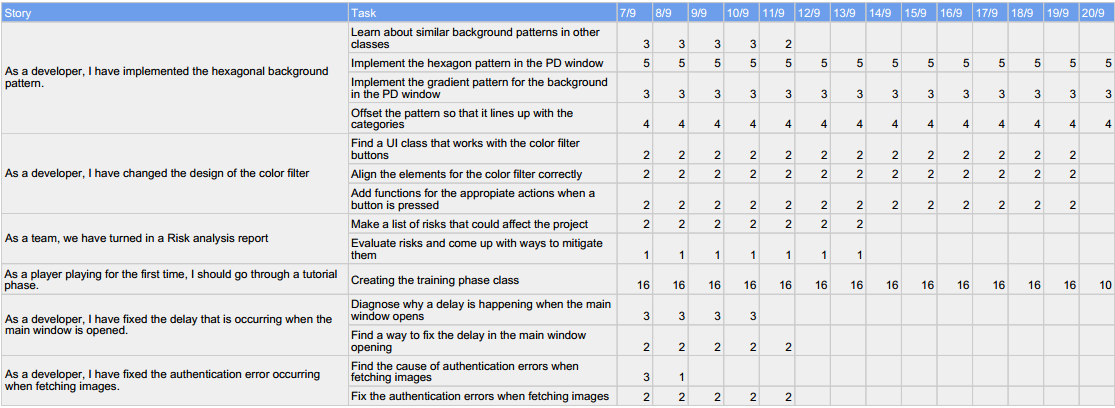
\includegraphics[scale=0.65]{sprint2.PNG}}
    \caption{\label{fig:s2}Sprint backlog for sprint 2}
\end{figure}

\begin{figure}[H]
	\centering
	\graphicspath{ {./graphics/} }
    \centerline{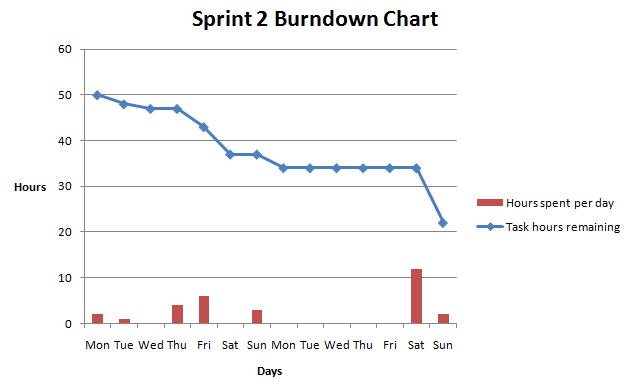
\includegraphics[scale=0.8]{sprint2bdc.PNG}}
    \caption{\label{fig:s2bd}Sprint burndown chart for sprint 2. The reason for no hours registered during the weekdays of the second week is that we used all our time on re-writing reports and preparing for the first status meeting.}
\end{figure}

\subsection{Sprint 3}
The theme of this sprint was working to finish the tutorial phase of the game and working on the website for the game. 

The things that went well during this sprint were that we got a clear idea on how the first version of the website should look and what content it should have. Development of the website also went well.  

As for the things that didn't go well, we were still suffering for the mistake we made in sprint 2 with the big story for the tutorial phase. We did not manage to finish the story in this sprint. We also had obligations in other courses that affected the time we were able to spend on the project, we only managed the bare minimum hours we had planned. 

\begin{figure}[H]
	\centering
	\graphicspath{ {./graphics/} }
    \centerline{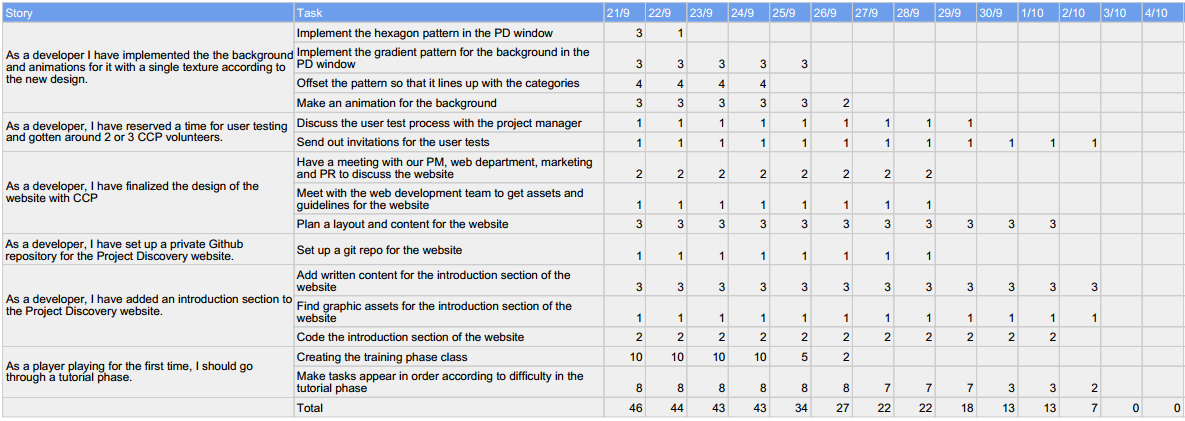
\includegraphics[scale=0.65]{sprint3.PNG}}
    \caption{\label{fig:s3}Sprint backlog for sprint 3}
\end{figure}

\begin{figure}[H]
	\centering
	\graphicspath{ {./graphics/} }
    \centerline{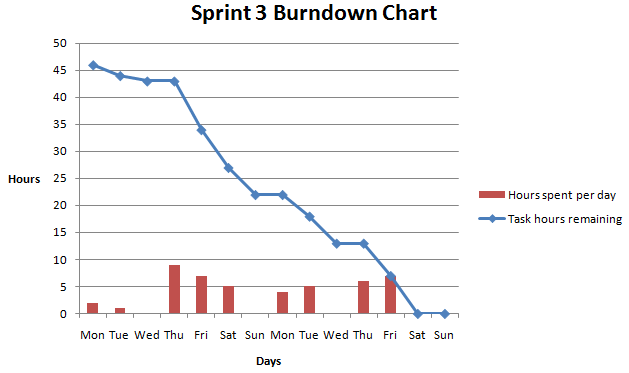
\includegraphics[scale=0.8]{sprint3bdc.PNG}}
    \caption{\label{fig:s3bd}Sprint burndown chart for sprint 3}
\end{figure}

\subsection{Sprint 4}
For the first week of this sprint we had a visit from our partner from MMOS, Attila Szantner. We therefore had a chance to work closely with him on the direction of the game. We committed ourselves to make good use of the time he spent here so we decided to spend much more time on the project than usual during this week. The theme of this sprint was a lot of meetings and shaping of the direction of the game. We met several times with Attila and various CCP employess during the week. We also performed a preliminary in-house user test by CCP request which was really useful in exposing things that need to be improved before the game can be launched on a test server.

The things that went well during this sprint were that we got a very clear idea on what needs to be done before the game goes out on a test server. We got great feedback from the user test which will be of immense help going forward. We also managed to be very productive with the extra time we spent on this sprint. We finally managed to finish the tutorial phase and we finished many other stories so our velocity for this sprint was exceptional compared to earlier sprints. That meant our average velocity was finally up to an acceptable standard.

The only thing that didn't go well during this sprint was all the time we spent on the project negatively impacted our progress in other courses at school, which might come back to haunt us later if we need to make up the time.

\begin{landscape}

\begin{figure}[H]
	\centering
	\graphicspath{ {./graphics/} }
    \centerline{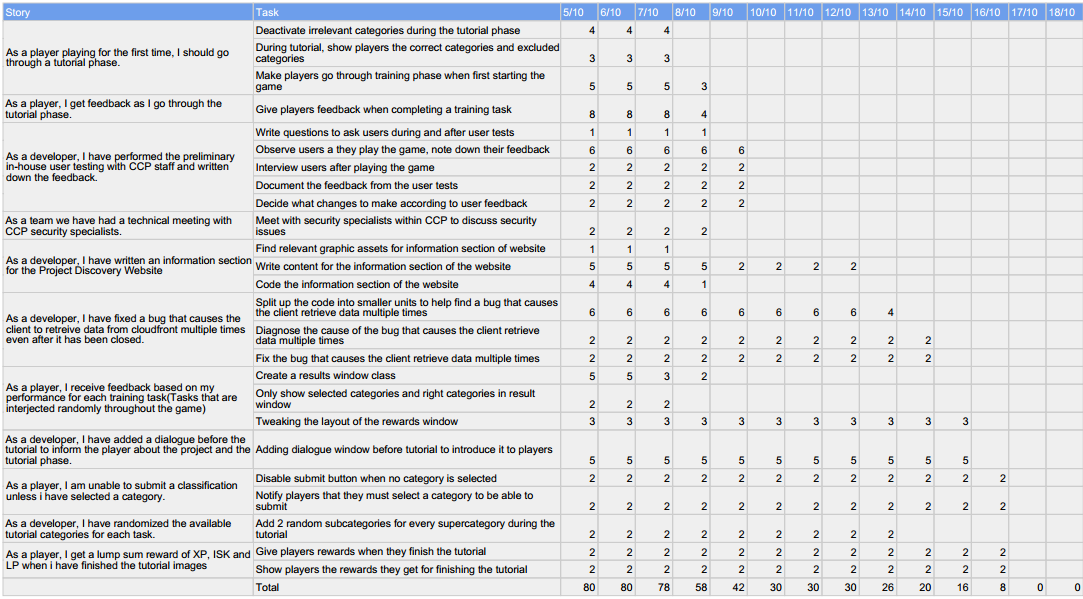
\includegraphics[scale=0.7]{sprint4.PNG}}
    \caption{\label{fig:s4}Sprint backlog for sprint 4}
\end{figure}

\end{landscape}

\begin{figure}[H]
	\centering
	\graphicspath{ {./graphics/} }
    \centerline{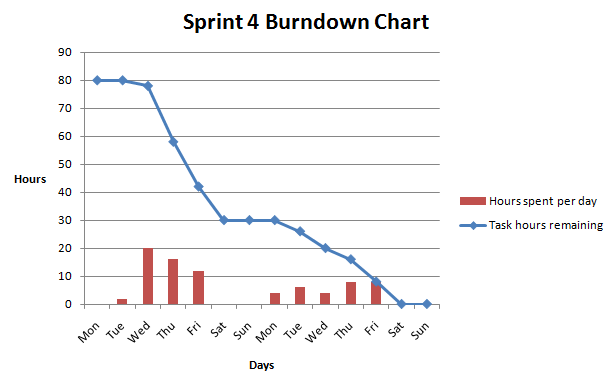
\includegraphics[scale=0.8]{sprint4bdc.PNG}}
    \caption{\label{fig:s4bd}Sprint burndown chart for sprint 4}
\end{figure}

\subsection{Sprint 5}

\subsection{Sprint 6}

\subsection{Sprint 7}